\chapter{Methodology}
\label{ch:Methodology}
This chapter outlines the technical methodology adopted in the development of the system, covering both low-level design and software implementation. The approach prioritizes performance, privacy, and modularity, leveraging hardware accelerators where possible and maintaining efficient control over data flow and execution.

%----------------------
\section{Retrieval-Augmented Generation (RAG) Pipeline}
\label{sec:RAGPipeline}
%----------------------

Retrieval-Augmented Generation (RAG) is an architectural framework designed to enhance the capabilities of language models by integrating external knowledge retrieval into the generation process \cite{lewis2020rag}. Unlike standalone LLMs that rely solely on pre-trained knowledge, RAG introduces dynamic document retrieval as part of the inference pipeline, thereby improving factual accuracy, contextual relevance, and grounding.

The RAG pipeline can be decomposed into modular phases, each responsible for a specific task in the information flow. The following subsections describe these phases and their associated components.

%----------------------
\subsection{Ingredients of a RAG (Retrieval-Augmented Generation) Application}
\label{subsec:IngredientsOfRag}
%----------------------

A Retrieval-Augmented Generation (RAG) system typically comprises four key components: \textbf{Document loader}, \textbf{Text embedder}, \textbf{Context retriever}, and \textbf{Response generator}. Both the Text embedder and the Response generator consist of a Language Model. As illustrated in Figure~\ref{fig:rag_overview}, documents are chunked, embedded, and stored in a vector database. This database is later queried to retrieve relevant context for a given user query, which is then passed along to the language model. This enables the model to generate responses grounded in a specific knowledge source, thereby enhancing the factual accuracy and credibility of the output.

The RAG pipeline can be conceptually divided into two major phases: \textbf{Embedding} and \textbf{Retrieval}.
\begin{figure}[h]
    \centering
    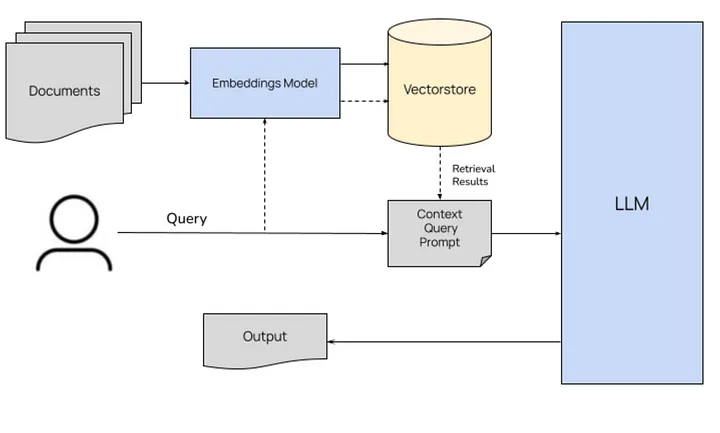
\includegraphics[width=0.75\textwidth]{images/RAG-pipeline.jpeg}
    \caption{High-level overview of a RAG system with its four main components~\cite{glenn2024mastering}}
    \label{fig:rag_overview}
\end{figure}

%----------------------
\subsection{Embedding Phase}
\label{subsec:EmbeddingPhase}
%----------------------

The embedding phase forms the foundation of a Retrieval-Augmented Generation (RAG) system by building the knowledge corpus that the system will later reference to answer user queries (Figure~\ref{fig:embedding_phase}). While the concept of text embeddings has existed since the introduction of Word2Vec in 2013 \cite{mikolov2013efficient}, their application for contextual storage and retrieval became prominent with the advent of \textit{in-context learning}, as introduced in the GPT-3 paper \cite{brown2020language}. This technique leverages the autoregressive nature of decoder-only transformers to generate relevant outputs based on few or even a single example \cite{bashir2023context}.

\begin{figure}[h]
    \centering
    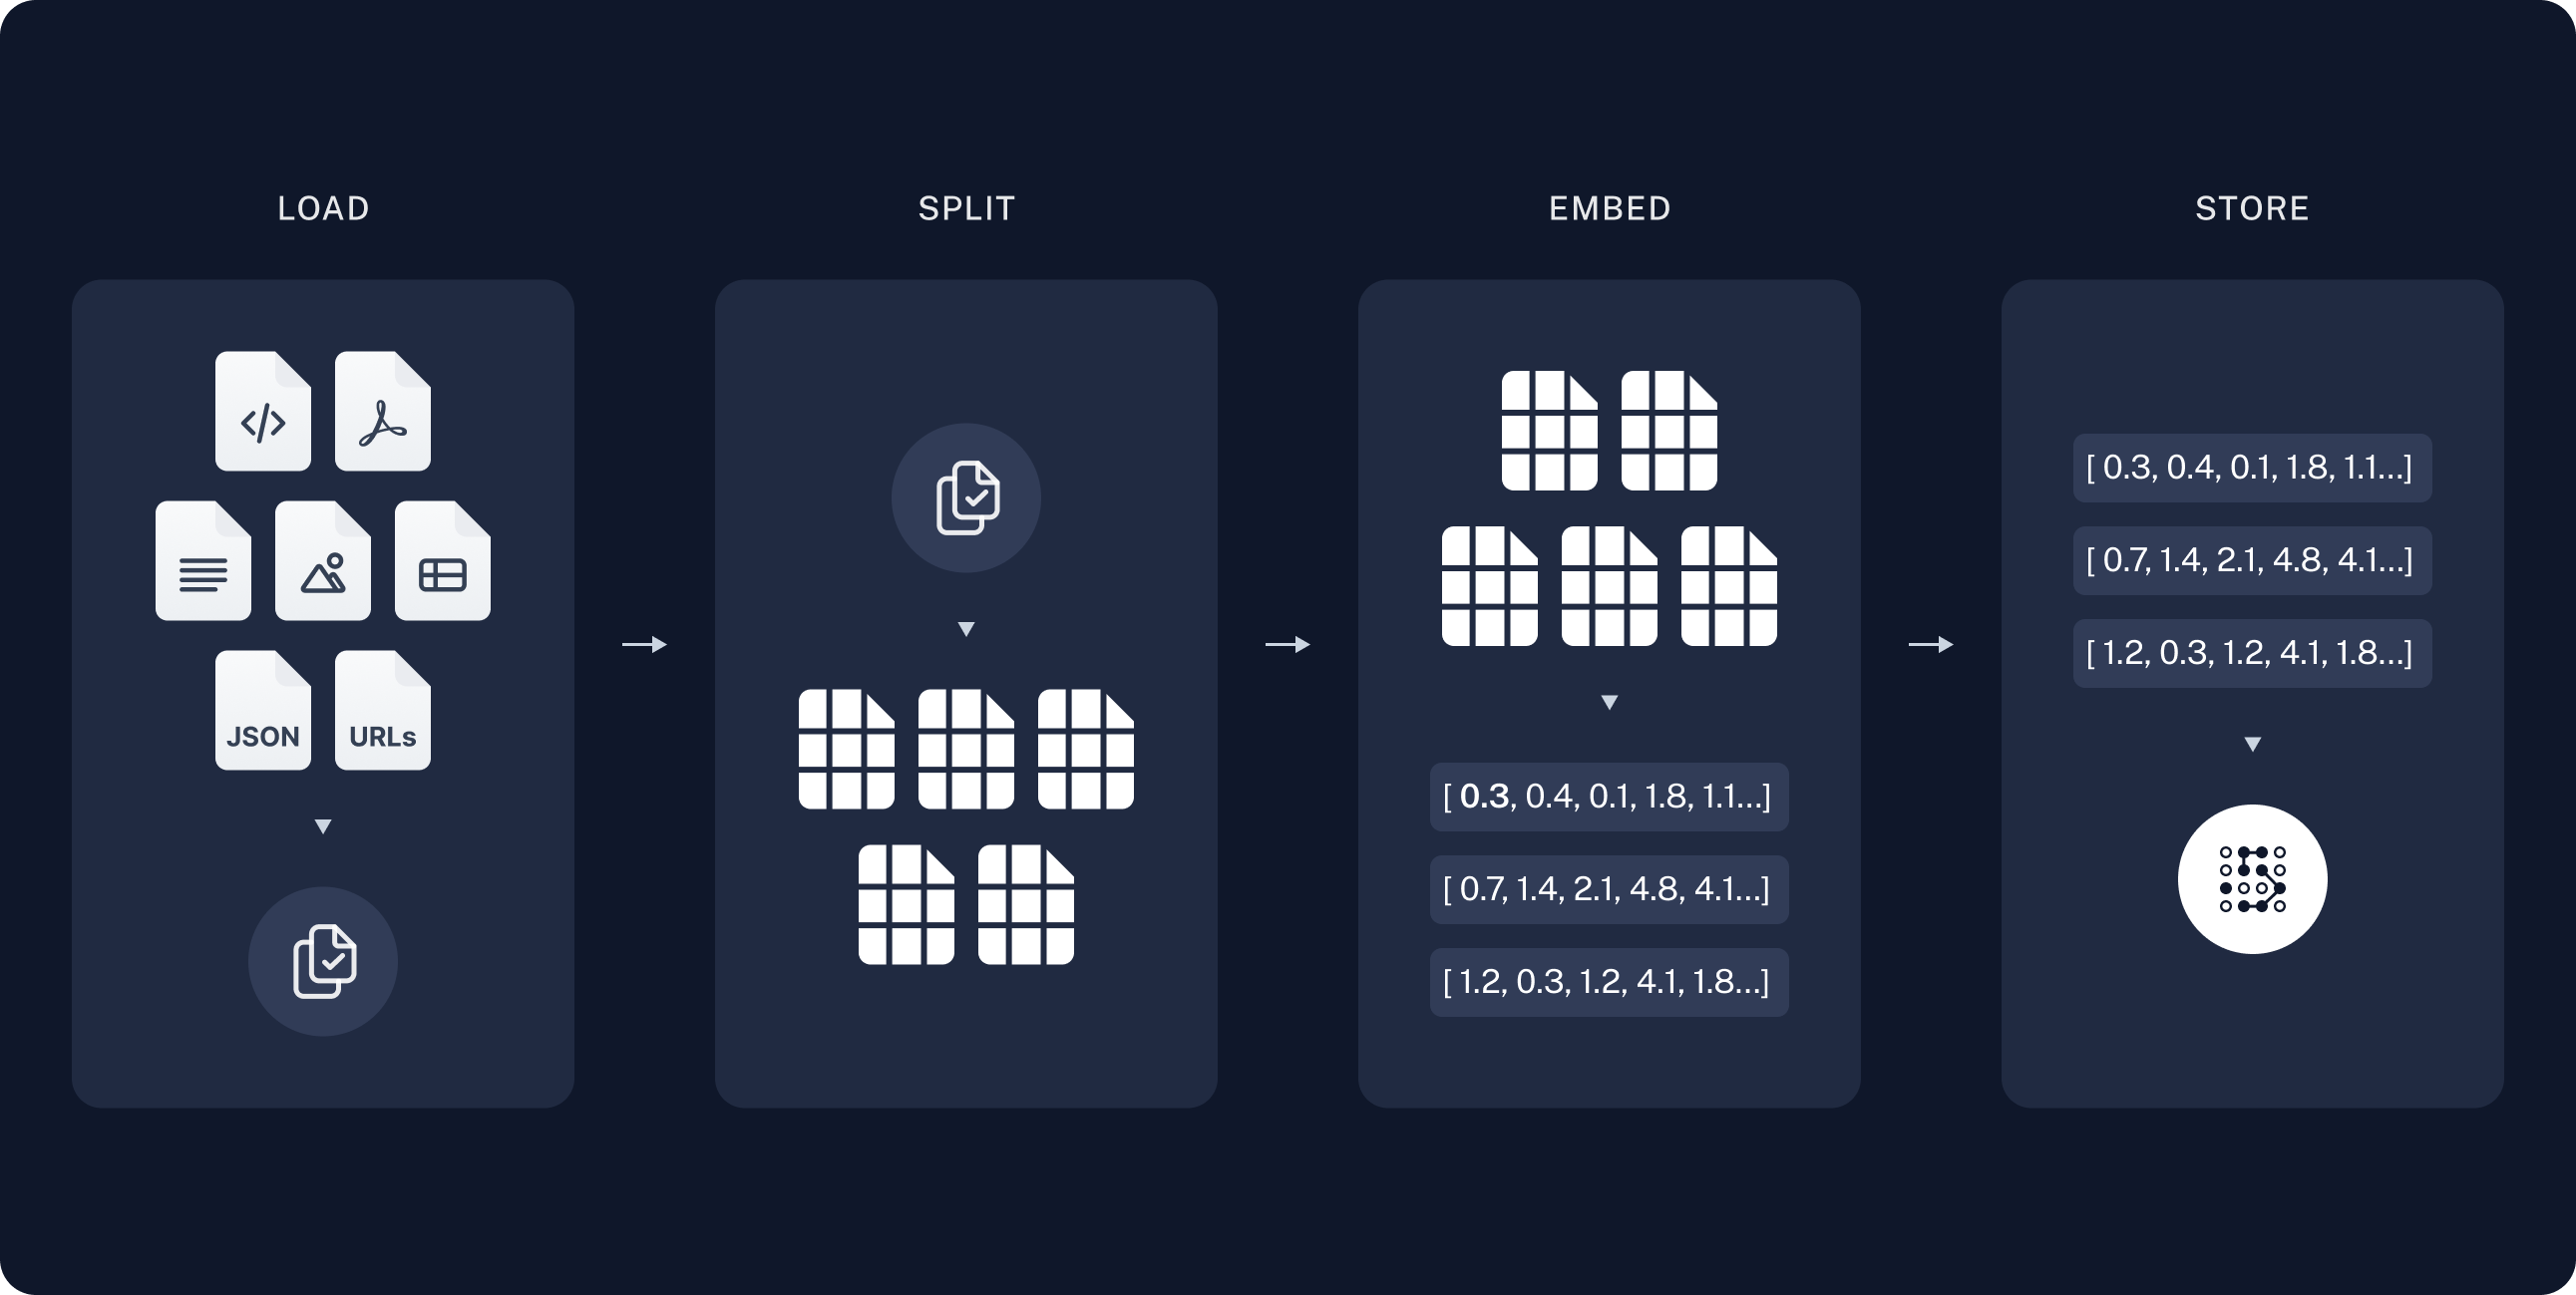
\includegraphics[width=0.75\textwidth]{images/lagchain-rag-embedding.png}
    \caption{The embedding phase: document ingestion, chunking, and vectorization~\cite{langchain_rag}}
    \label{fig:embedding_phase}
\end{figure}

The embedding phase comprises several key steps:

\begin{enumerate}[label=\alph*.]
  \item \textbf{Document Processing:} Documents in formats such as TXT, PDF, or DOCX are loaded. This may be done in text-only or multi-modal modes, the latter preserving diagrams and figures. This task is handled by the Document Loader module.

  \item \textbf{Chunking:} The loaded documents are split into smaller, semantically coherent segments using text splitters \cite{langchain2023textsplitters}. Chunking is necessitated by the limited context window of LLMs, which ranges from 2K tokens in GPT-3 to 128K tokens in LLaMA 3 \cite{touvron2024llama3}. Moreover, using large contexts also demands significant GPU memory, especially when optimizations like KV caching and speculative decoding are employed.

  Improper chunking can impair performance:
  \begin{itemize}
    \item \textit{Chunks too large} may result in the ``Lost in the Middle'' effect \cite{liu2023long}, where only the beginning and end of the chunk influence the output.
    \item \textit{Chunks too small} lead to redundancy and latency, as overlapping content is required to preserve context.
  \end{itemize}

  \item \textbf{Chunking Techniques:}
  \begin{itemize}
    \item \textbf{Length-based chunking:} Divides text based on fixed token or character length. Tokens are determined using subword tokenization techniques like byte-pair encoding \cite{sennrich2015neural}.
    \item \textbf{Semantic chunking:} Splits based on document structure, e.g., paragraphs.
    \item \textbf{Context-aware splitting:} Ensures that subtopics are not broken across chunks.
  \end{itemize}

  In some approaches, particularly token count or context-aware chunking, embedding may precede the splitting step.

  \item \textbf{Text Embedding:} In this step, each chunk is converted into a dense vector using a text embedding model. The embedding model used here does not need to match the LLM used in generation, as the embeddings are utilized solely for vector similarity search. Once relevant chunks are retrieved, their original textual content is passed to the LLM, not the embeddings themselves. Compact and efficient models like BERT or DistilBERT are often employed for this task due to their relatively small embedding sizes (e.g., 512 or 768 dimensions), which makes them computationally lightweight compared to models like LLaMA \cite{touvron2023llama} or GPT-3 \cite{brown2020language}, which produce larger embeddings in the range of 1024 to 12,288 dimensions. Although these smaller embeddings may be less precise, they are generally sufficient for high-level semantic retrieval.
\end{enumerate}

%----------------------
\subsection{Retrieval Phase}
\label{subsec:RetrievalPhase}
%----------------------

The retrieval phase is initiated whenever a user submits a query or task. This phase makes use of the vector database constructed during the embedding phase to locate and extract relevant content for the given input prompt, which is then passed to the language model for response generation (Figure~\ref{fig:retrieval_phase}).



\begin{figure}[h]
    \centering
    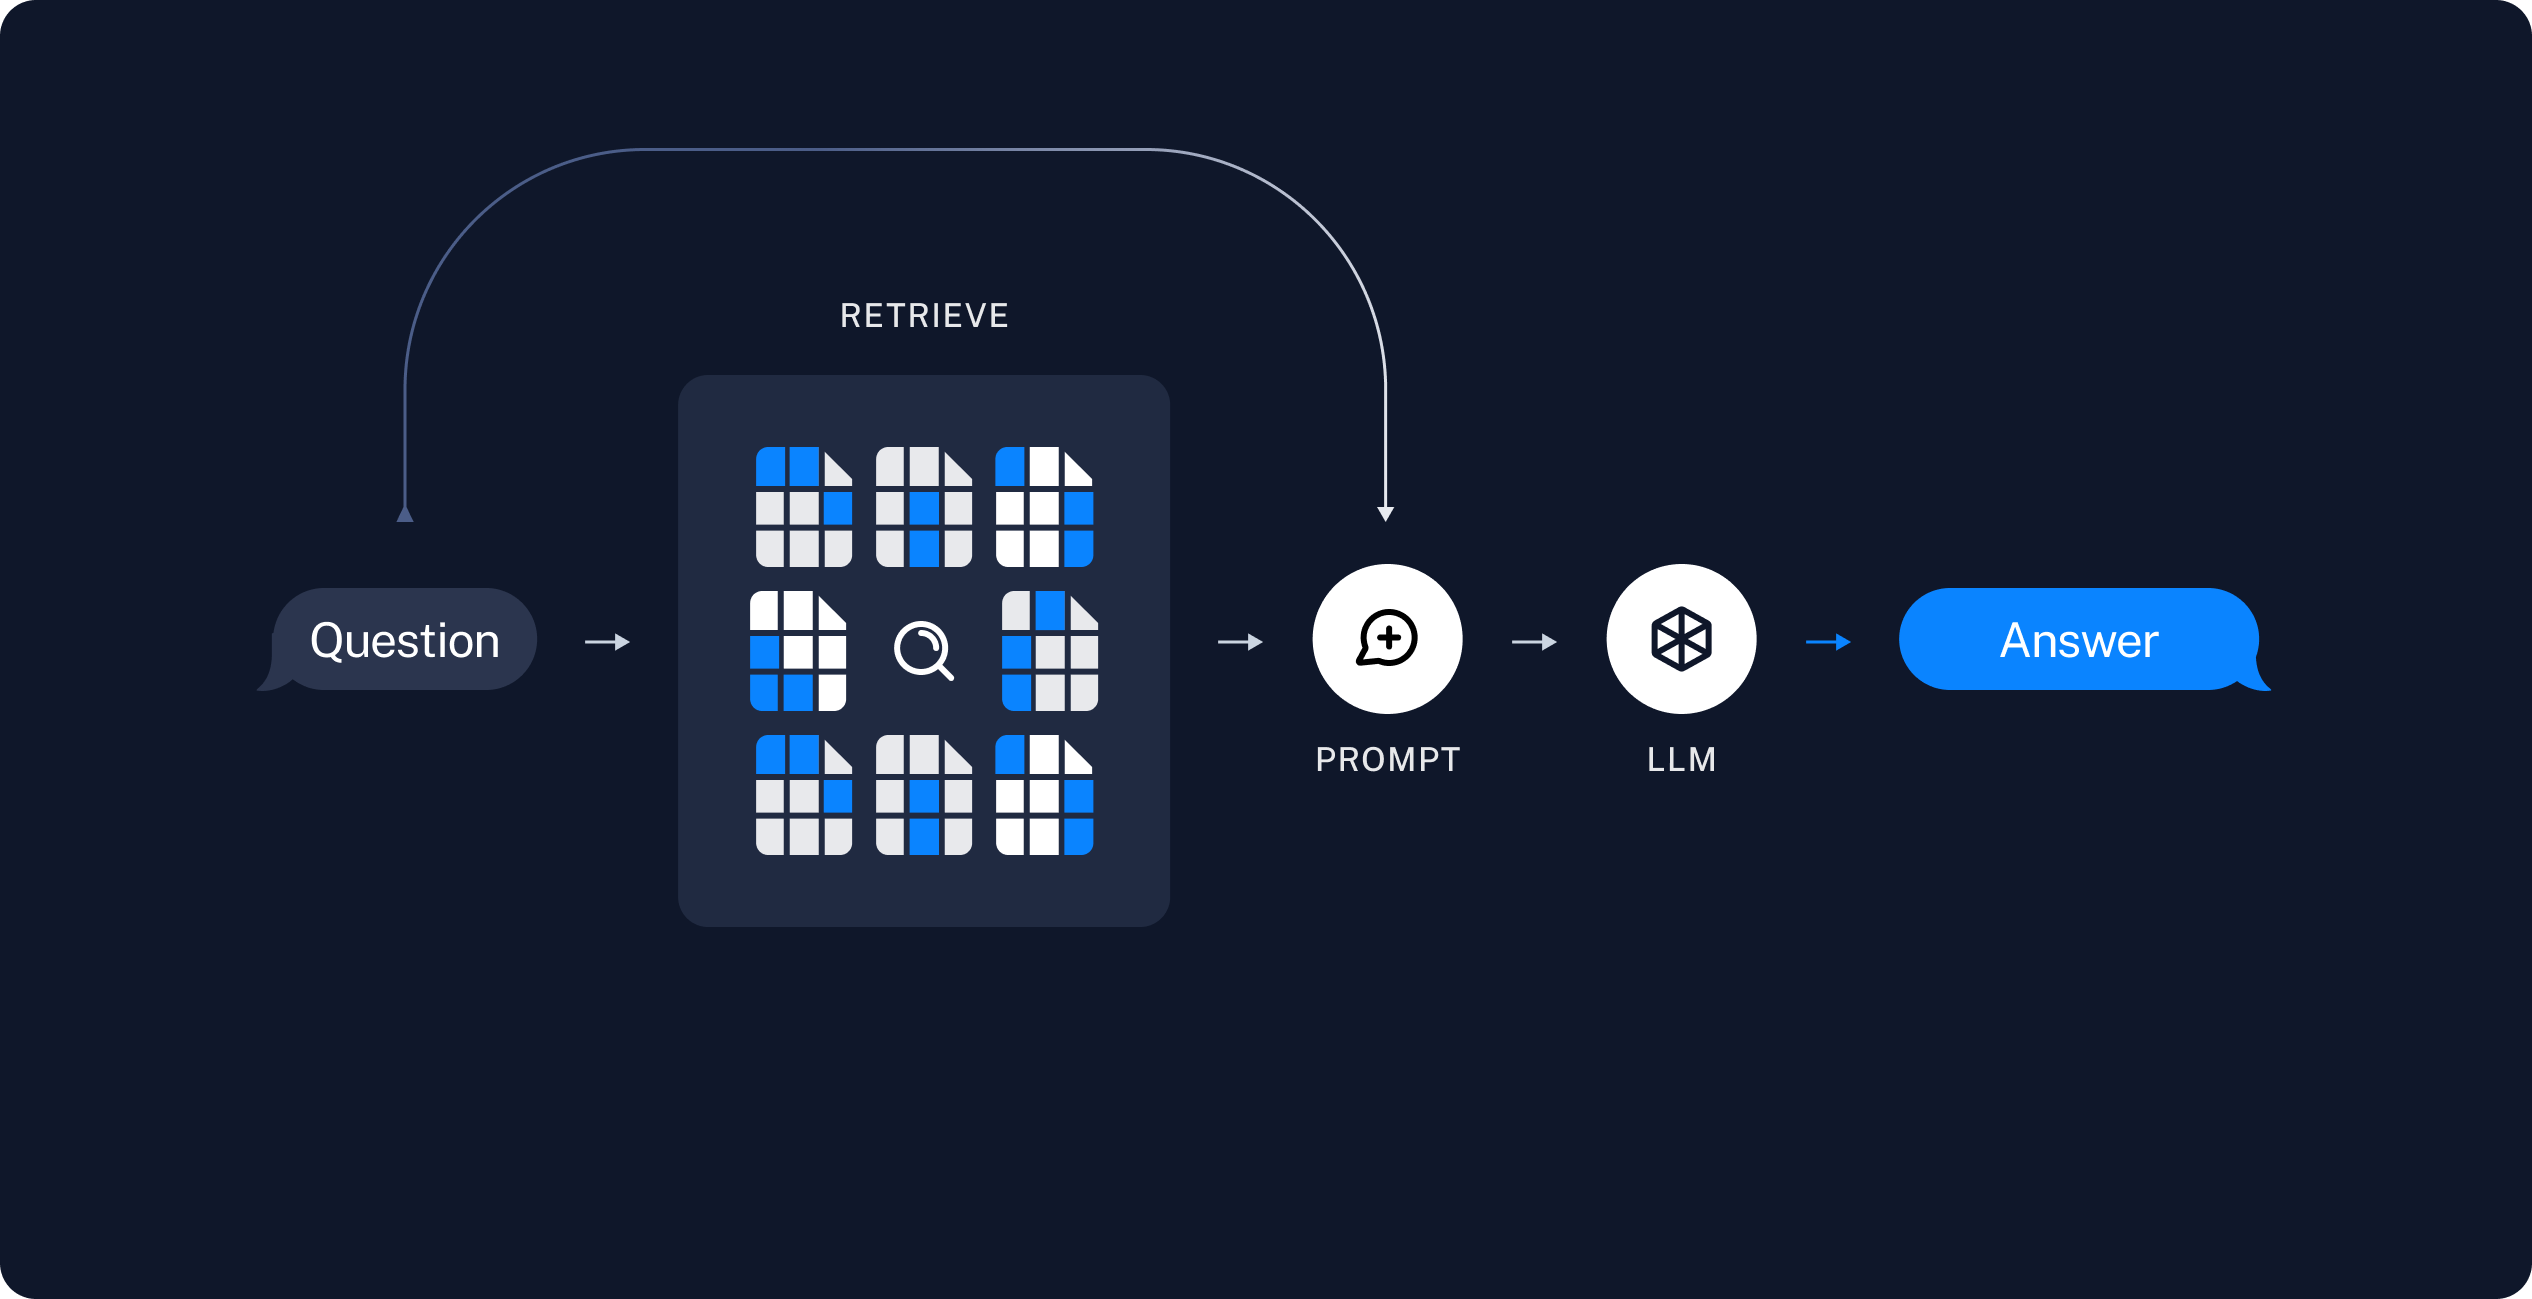
\includegraphics[width=0.75\textwidth]{images/lagchain-rag-retrieval.png}
    \caption{The retrieval phase: querying the vector store and invoking the LLM~\cite{langchain_rag}}
    \label{fig:retrieval_phase}
\end{figure}

\begin{enumerate}[label=\alph*.]
  \item \textbf{Context Retrieval:} The context retriever module follows a two-step process:
  \begin{enumerate}
    \item Embedding the user's query using the same embedding model employed during the embedding phase.
    \item Performing a similarity search in the vector database to identify top-matching chunks based on the embedded query.
  \end{enumerate}

  The quality of similarity search is crucial, as it directly impacts the relevance and accuracy of the LLM-generated response. In the embedding space, proximity denotes semantic similarity—closer vectors imply greater contextual relevance. However, efficient neighbor discovery in high-dimensional vector space is computationally expensive, and full database scans are often impractical \cite{sugawara2016approxsearch}.

  \item \textbf{Search Algorithms:} To balance accuracy, latency, and resource usage, the following approximate nearest neighbor (ANN) algorithms are commonly employed:
  \begin{enumerate}
    \item \textbf{Cosine Similarity Search:} Measures the cosine of the angle between vectors to determine their similarity. It is widely used in embedding-based retrieval tasks due to its scale invariance and intuitive geometric interpretation. This is \textit{highly parellizable} and simple to implement. \cite{steck2024cosine}. 
    This is project primarily relies on cosine similarity for embedding retrieval.
    
    \item \textbf{k-Nearest Neighbors (kNN):} A brute-force method that identifies the $k$ closest vectors through exhaustive comparisons~\cite{labelbox2023vectorsimilarity}.
    
    This project uses kNN as a fallback mechanism to search in the database using pg-vector~\cite{pgvector}. 
    
    
    \item \textbf{Locality-Sensitive Hashing (LSH):} Hashes vectors into buckets such that similar vectors are likely to fall into the same bucket \cite{labelbox2023vectorsimilarity}.
    \item \textbf{k-d Trees:} Uses recursive partitioning of the embedding dimensions to index and query data \cite{labelbox2023vectorsimilarity}.
    \item \textbf{HNSW (Hierarchical Navigable Small World) Graphs:} Constructs a layered graph to enable fast traversal through neighbors across different granularity levels \cite{labelbox2023vectorsimilarity}.
    \item \textbf{ScaNN (Scalable Nearest Neighbors):} A Google-designed ANN method that integrates pruning, quantization, and partitioning for scalable, memory-efficient retrieval \cite{guo2020accelerating}.
  \end{enumerate}

\begin{figure}[H]
    \centering
    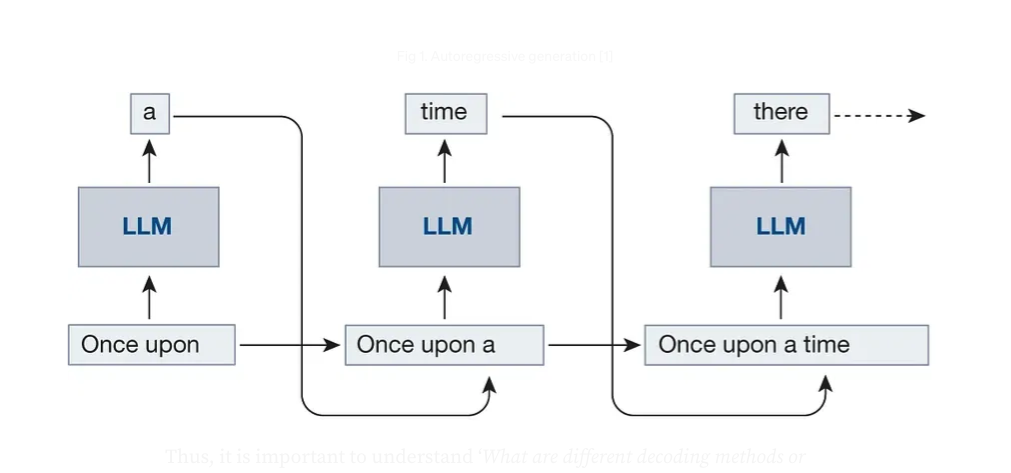
\includegraphics[width=0.6\linewidth]{images/autoregressive-decoding.png}
    \caption{Autoregressive decoding ~\cite{nabi2024all}}
    \label{fig:autoregressive_decoding}
\end{figure}

\item \textbf{Output Generation:}
In this phase, the retrieved context and the user input—both in plain text form—are fed into the Large Language Model, as illustrated in Figure 1.3. The LLM processes the portion of input that fits within its context window and generates an output token. This token is then concatenated with the input and passed back to the LLM. The process repeats iteratively until the LLM produces an <EOS> (end-of-sequence) token.


\end{enumerate}

\subsection{Output Evaluation:}
The evaluation of a Retrieval-Augmented Generation (RAG) system focuses on the quality of the output in terms of its relevance to the user's query and the information stored in the vector database. Since different components contribute uniquely to the overall performance, multiple metrics are used rather than a single aggregated score to allow for precise attribution and targeted optimization.

Classical metrics such as Precision, Recall, and F1 score, alongside NLP-specific metrics like ROUGE, are employed to assess performance. The evaluation considers several factors, as illustrated in Figure 1.5:
\begin{itemize}
    \item \textbf{Faithfulness, Output Relevance \& Semantic Similarity:} Measures the quality of the output relative to the input queries and retrieved context.
    \item \textbf{Context Recall \& Context Precision:} Assess the effectiveness of context retrieval and its utilization by the LLM.
\end{itemize}
\begin{figure}[H]
    \centering
    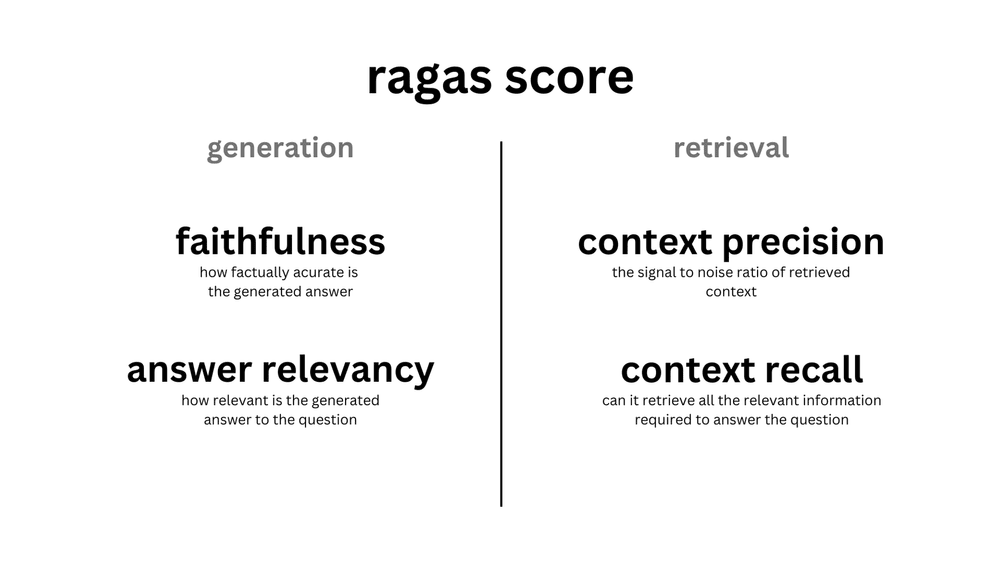
\includegraphics[width=0.56\linewidth]{images/rag-eval.png}
    \caption{RAG Output evaluation metrics ~\cite{cardenas2023rag}}
    \label{fig:autoregressive_decoding}
\end{figure}



%----------------------
\section{II. Application Design}
\label{sec:II.ApplicationDesign}
%----------------------
\begin{figure}[H]
    \centering
    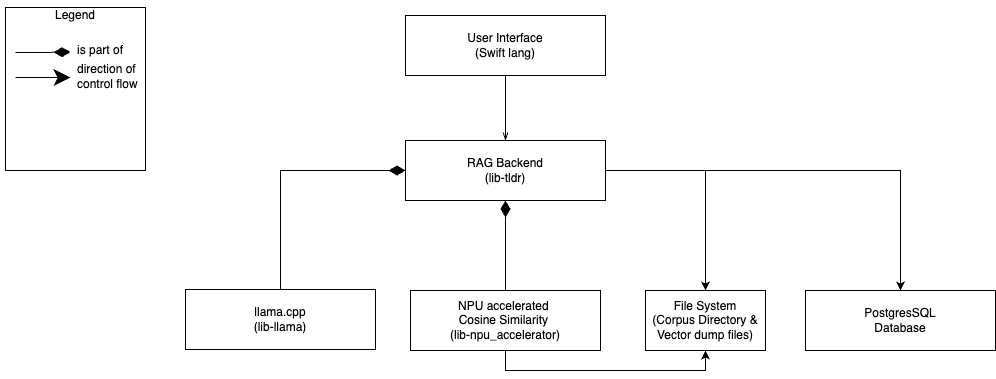
\includegraphics[width=1.0\linewidth]{images/tldr-app-modules.png}
    \caption{RAG Output evaluation metrics ~\cite{cardenas2023rag}}
    \label{fig:autoregressive_decoding}
\end{figure}


\begin{figure}[H]
    \centering
    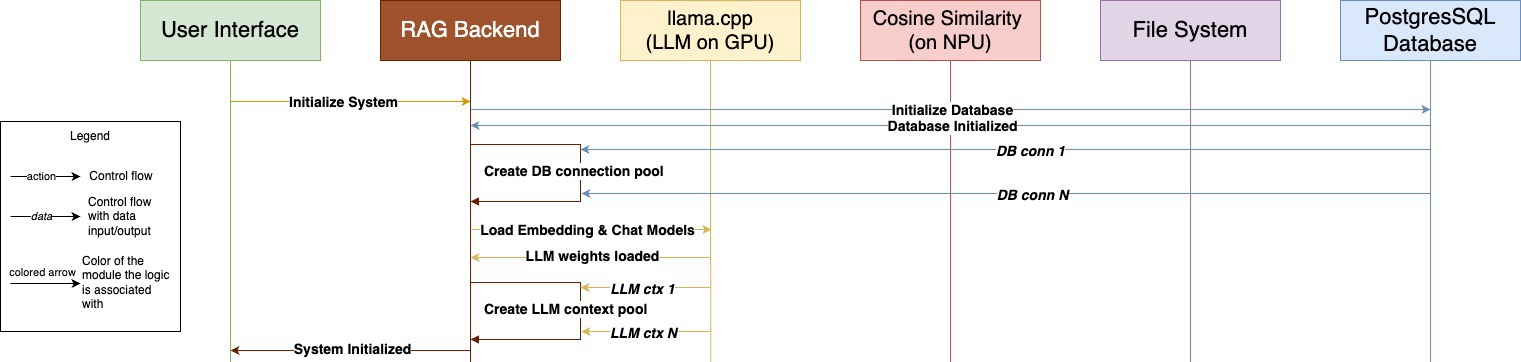
\includegraphics[width=1.0\linewidth]{images/tldr-app-worklfow-pt1.jpg}
    \caption{RAG Output evaluation metrics ~\cite{cardenas2023rag}}
    \label{fig:autoregressive_decoding}
\end{figure}

\begin{figure}[H]
    \centering
    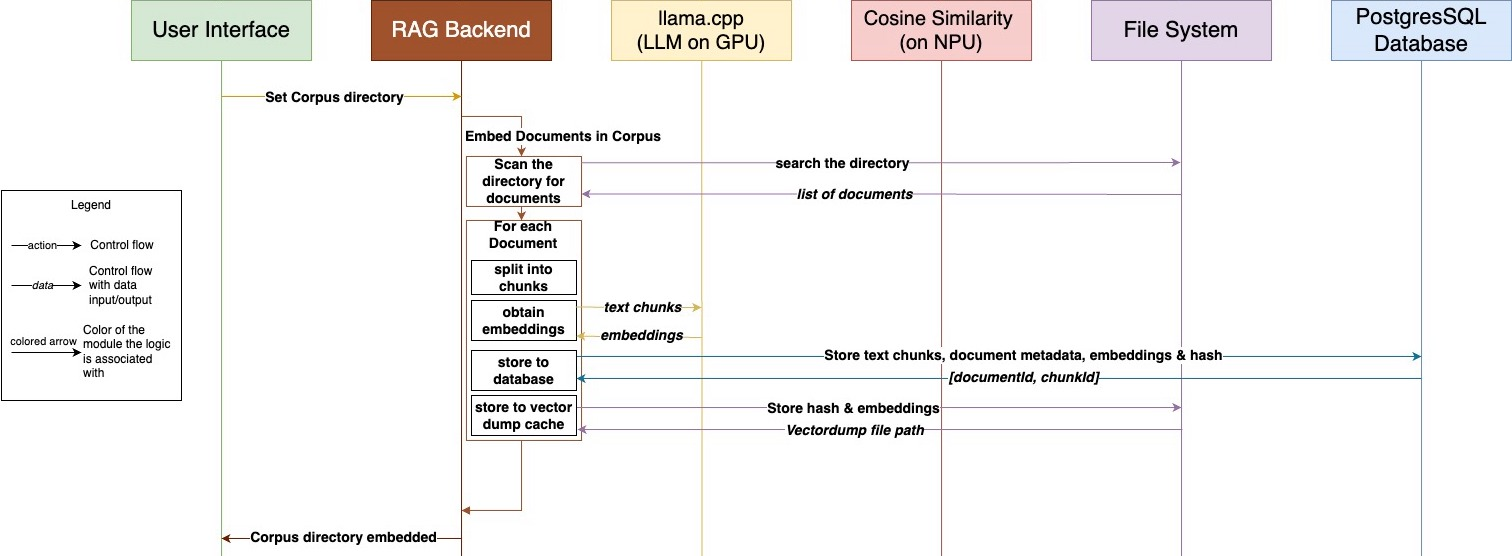
\includegraphics[width=1.0\linewidth]{images/tldr-app-worklfow-pt2.jpg}
    \caption{RAG Output evaluation metrics ~\cite{cardenas2023rag}}
    \label{fig:autoregressive_decoding}
\end{figure}

\begin{figure}[H]
    \centering
    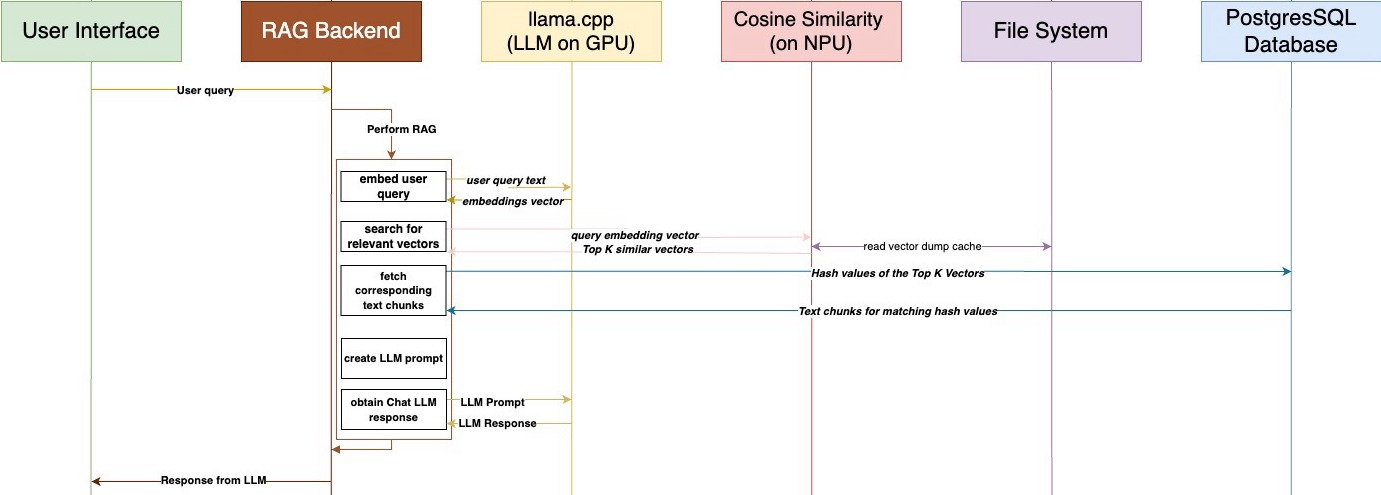
\includegraphics[width=1.0\linewidth]{images/tldr-app-worklfow-pt3.jpg}
    \caption{RAG Output evaluation metrics ~\cite{cardenas2023rag}}
    \label{fig:autoregressive_decoding}
\end{figure}


%----------------------
\section{III. Application Implementation}
\label{sec:III.ApplicationImplementation}
%----------------------
